\chapter{Realizability of Entropy}\label{chapter:krieger}

In this chapter we finally combine various tools developed throughout this thesis to deduce its two main results: the realizability of entropy for minimal subsystems and proximal subsystems. 
%
We hope that the theory developed around these tools in the previous chapters is already interesting by itself. It is this particular application that indicates that this theory is also useful and allows to both obtain new, simpler proofs of old results and to prove new theorems.

\section{Minimal Subsystems}
In this section, we show that each possible finite value of entropy is realizable by some minimal dynamical subsystem of $\alf^G$ assuming only that $G$ is a congruent monotilable group.
%
Recall that this result was initially proved by Krieger \cite{Krieger07} and later reproved by \cite{LS18} assuming that the group $G$ is residually finite.
%
Our generalization  includes in particular all virtually nilpotent and all abelian groups; perhaps the simplest example that is captured now, but was not previously is $(\Q, +)$ (the additive group of rationals).

Recently, it was brought to author's attention that a result by Rosenthal in an unpublished  manuscript\footnote{The author would like to thank Dominik Kwietniak and Benjamin Weiss for obtaining a copy of this manuscript.}  \cite{Rosenthal} might likely be used to give a different proof of the Theorem \ref{Krieger2}.  
%
Specifically, Rosenthal's main theorem asserts that if $(Y,\Sigma,\nu)$ is a standard probability space with a free ergodic measure preserving action of an amenable group $G$, then there exists a compact
metric space $X$ and an action of $G$ on X preserving a Borel probability measure $\mu$ such that $(X,G)$ is a minimal dynamical system and $\mu$ is unique measure invariant for the action of $G$ on $X$. 
%
Furthermore, the ergodic measure preserving action of $G$ on $X$ is isomorphic with the action of $G$ on $Y$.
%
While the theorem does not specify what the space $X$ is, one might try to repeat the proof (thus also go through the argument of \cite{HR73}, \cite{Rosenthal89} and \cite{Weiss85}) associating with $Y$ a minimal subshift of $\{0,1,\ldots,d-1\}^G$ whenever the Kolmogorov-Sinai entropy of $(Y,\nu,G)$ is strictly smaller than $\log d$.

\begin{thm}[Realizability of entropy for minimal systems]\label{Krieger2}
Let $G$ be a congruent monotliable group and $\alf$ be a finite alphabet. Then  for every number $\gamma\in[0,1)$ there exists a minimal subsystem $Y$ of the dynamical system $(\alf^G,G)$ such that $\htop(Y)=\gamma\log |\alf|$.
\end{thm}


\begin{proof}
We show that for every number $\gamma \in [0,1)$ there exists an element $x\in \alf^G$ being a quasi-Toeplitz configuration such that
\begin{equation}\label{eq:exists_qt}
h(x) = \htop(\closure{Gx}) = \gamma \log |\alf|.
\end{equation}
Having established that,  to conclude the Theorem it is enough to apply Lemma~\ref{lem:toeplitz-minimal} which says that each such subsystem $\closure{Gx}$ is minimal.

To prove existence of an $x$ satisfying~\eqref{eq:exists_qt} for every $\gamma \in [0,1)$ we use the properties of quasi-Toeplitz sequences that we have established in previous chapters.
%
First of all, by Lemma~\ref{lem:connected2} the space of quasi-Toeplitz configurations is path-connected with respect to the Weyl pseudometric.
%
Secondly, as proved in Theorem~\ref{thm:shift_entropy_cont}, the entropy function $h: \alf^G \to [0, \log |\alf|)$  is continuous on $\alf^G$ (when equipped with the Weyl pseudometric).
%

Therefore, it is enough to find a quasi-Toeplitz configuration that has entropy $0$ and then to find another quasi-Toeplitz configurations that have entropy arbitrarily close to $\log |\alf|$.
% 
The former is simple: the constant configuration $a^G$ for any $a\in \alf$ is clearly quasi-Toeplitz and has entropy $0$.
%
To show the latter, let us fix any $\gamma\in(0,1)$, we show that there exists a quasi-Toeplitz configuration $x\in\alf^G$ such that $h(x)\geq\gamma\log|\alf|$. 
%
To this end, let $\{F_n\}_{n\in\N}$ be a congruent \Folner sequence with the associated \elegant sequence $\mC=\{C_n\}_{n\in\N}$. Passing to a subsequence if necessary, we may assume that $$|F_{n+1}|\geq |F_n||\alf|^{|F_n|}.$$ For any $n\in\N$ we let 
\[
r_n\defeq\left\lfloor (1-\gamma)\frac{|F_n|}{2^{n+1}}\right\rfloor.
\] 
We construct a sequence $\{G_n\}_{n\in\N}$ of subsets of $G$ satisfying:
\begin{enumerate}
\item $G_n\subseteq F_n$ and $|G_n|=r_n$ for every $n\in\N$,
\item  $\displaystyle G_i\cap G_jC_j =\emptyset$ for $i\neq j,$
\item\label{cond3} $\displaystyle\bigcup_{n\in\N } G_nC_n=G.$
\end{enumerate}

Since $G$ is countable, we can enumerate its elements as $g_1, g_2, g_3,\ldots$.
%
Moreover, since $F_0 \subseteq F_1 \subseteq F_2 \subseteq \ldots$ and $\bigcup_{n\in \N} F_n = G$, we can make sure that the enumeration is ``consistent'' with the \Folner sequence $\{F_n\}_{n\in \N}$, i.e., whenever $g_i \in F_n$ and $g_j \in F_k \setminus F_n$ for some $n<k$ then $i<j$. 

The construction of $G_0,G_1,\ldots$ is inductive. Intuitively, $G_n$ is taken to be $r_n$ elements with smallest indices that do not appear in any ``shift'' of a previously selected subset $G_i$ (for $i<n$), i.e., not in $G_iC_i$ (for any $i<n$). One can imagine this process of constructing $G_0,G_1,\ldots$ as starting with the entire sequence $g_1,g_2,g_3,\ldots$ and then whenever $G_n$ is constructed, all its elements along with all their shifts by $C_n$ (i.e. $G_nC_n$) are erased from the sequence.

To formalize the above, define 
\[
G_0 \defeq \{g_1,\ldots, g_{r_0}\}\subseteq F_0.
\]
Now, assuming that $G_n$ is already constructed, $G_{n+1}$ is chosen to be 
\[
G_{n+1} \defeq \{g_{k_1},\ldots, g_{k_{r_{n+1}}}\},
\]
where 
\[
k_j \defeq \min\left\{i : g_i\notin \bigcup_{k=0}^nG_kC_k ~\mbox{ and }~ g_i \neq g_{k_l} \mbox{ for every } l=1,2, \ldots, j-1\right\}.
\]
 Now we construct $x\in\alf^G$ inductively as follows. 
 %
We start by setting $x_{F_0}$ arbitrarily.
%
Subsequently, we copy the ``pattern'' at $G_0\subseteq F_0$ on all shifts of $G_0$ by $C_0$, that is for every $g\in G_0$ and $c \in C_0$ we set $x(gc):= x(g)$.
%

We now describe the induction step: fix any $n\in \N$, after steps $0,1,\ldots, n$ we are left with $x$ defined  on the set $F_n \cup T_n \subseteq G$, where 
 \[
 T_n\defeq\bigcup_{j=0}^n G_jC_j.
 \] 
The goal is now to define $x$ on the remaining part of $F_{n+1}$.
%
Let $J_n$ be the subset of $C_n$ such that
$$F_{n+1} = \bigcup_{c\in J_n} F_n c.$$
Each such ``translated'' monotile $F_nc$ for $c\in J_n$, $c\neq e$, has a small part of it already filled (that is, $x$ is defined for $g$ in $F_nc\cap T_n$), but the remaining $|F_n \setminus T_n|$ elements of $F_nc$ are still to be set.
%
The idea is now to exhaust all $|\alf|^{|F_n \setminus T_n|}$ possible patterns (see Figure \ref{fig:krieger_construction}) over copies of $F_n$ when filling $F_{n+1}$.
%
Since by the choice of the \Folner sequence, $|J_n|\geq |\alf|^{|F_n|}$, this is indeed possible.
%
Having $x$ defined over $F_{n+1}$, as previously, we copy the part over $G_{n+1}$ over the whole group, formally for every $g\in G_{n+1}$ and $c\in C_{n+1}$ we put $x(gc):= x(g)$.
%
Now $x$ is defined over $F_{n+1} \cup T_{n+1}$.

\begin{figure}
\centering
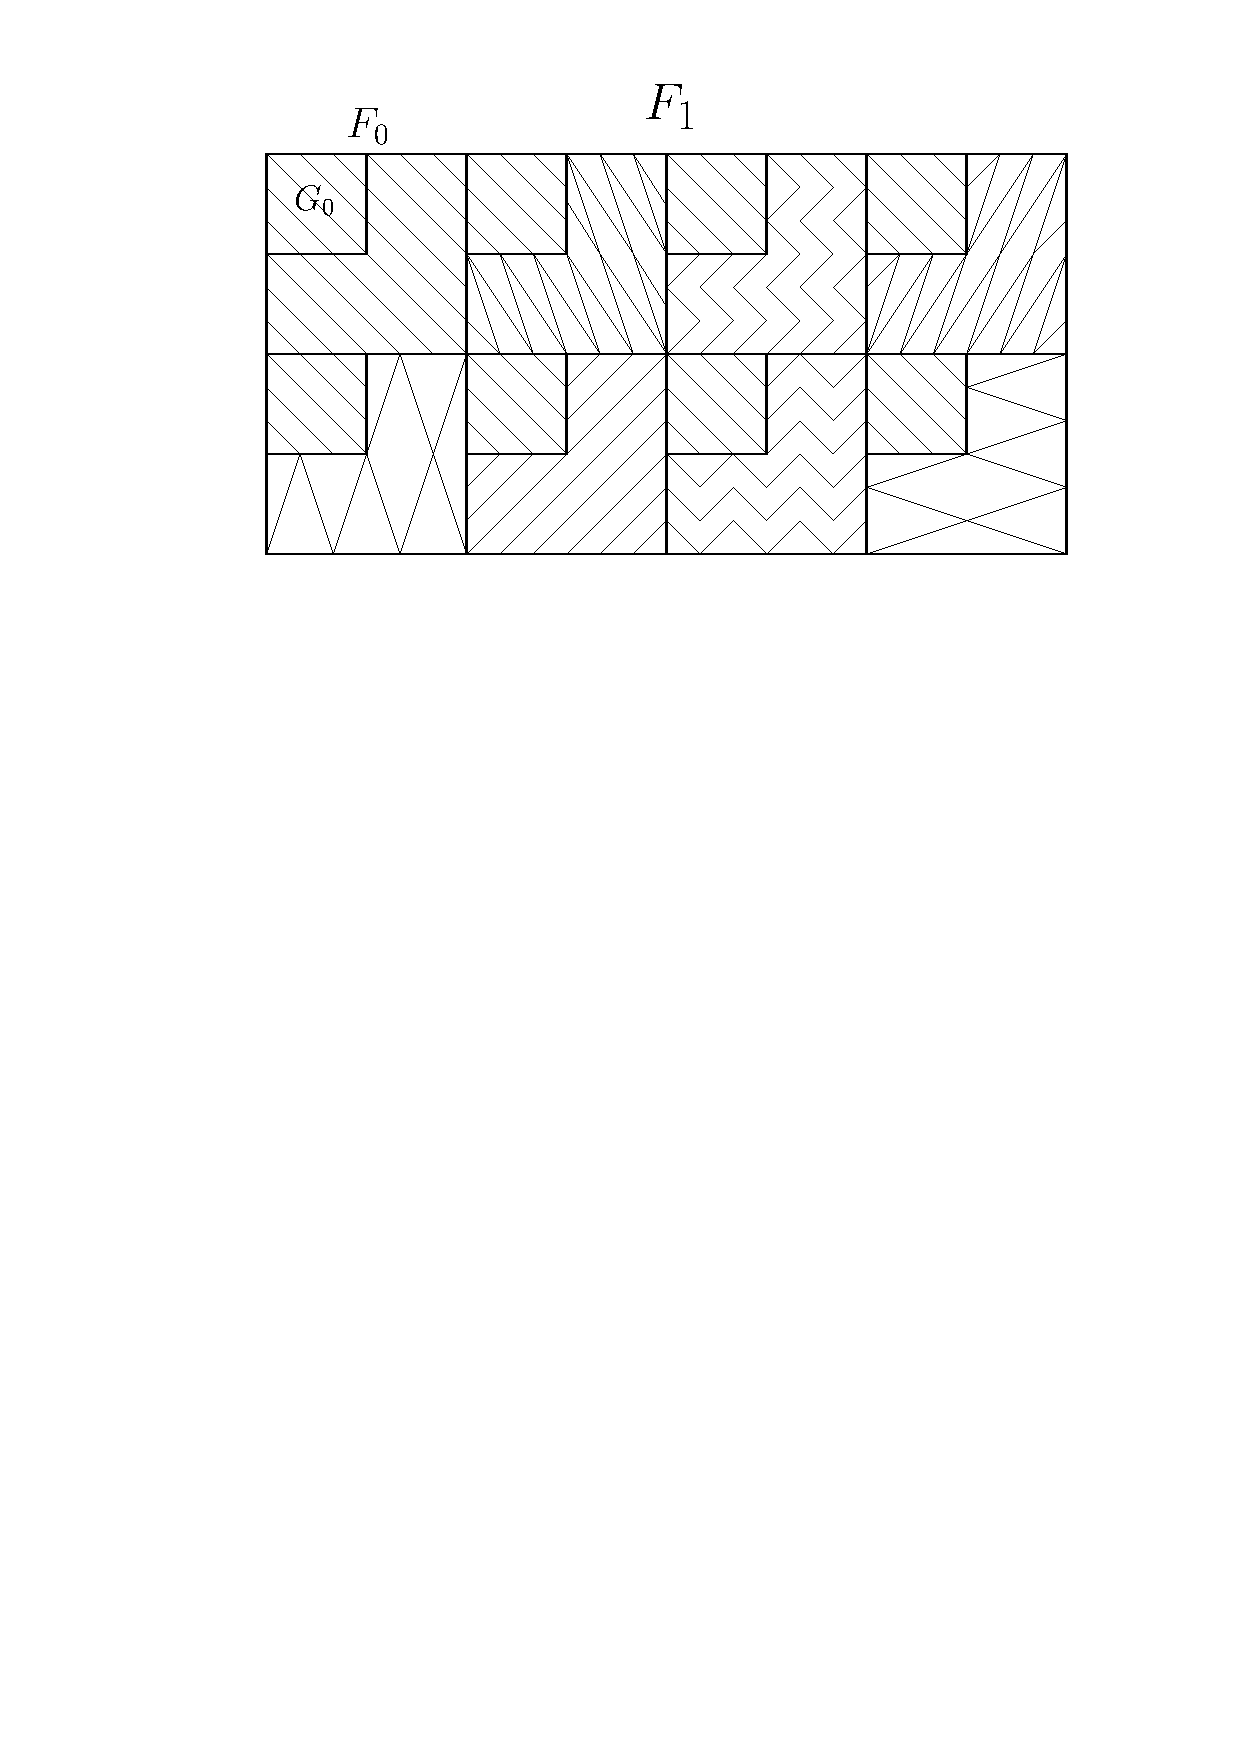
\includegraphics[scale=1]{../Graphics/krieger_construct}
\caption{One step of the construction of a Toeplitz sequence $x\in\alf^G$  from the proof of Theorem \ref{Krieger2}. In the $0$-th step we fill $F_0$ with arbitrary pattern, let's say diagonal lines, and copy this pattern from $G_0$ to the all group shifting it by elements from $C_0$. Next we fill the remaining place in $F_1$ as follows: assume that $|\alf|^{|F_0\setminus G_0|}=8$. That means that there are eight possibilities to fill the remaining place over the copies of $F_0$ in $F_1$ and we have just so many copies of $F_0$ in $F_1$. Therefore we fill each copy of $F_0\setminus G_0$ in $F_1$ with a different pattern.}\label{fig:krieger_construction}
\end{figure}

Having described the construction we are ready to prove the desired properties of $x$.
%
First of all, note that $x$ is a well-defined quasi-Toeplitz configuration; condition \ref{cond3} ensures that $x$ is defined at every index $g\in G$ and ``all its elements are quasi-periodic''.

The next step is to bound the entropy of $x$ from below. To this end, recall that in the construction of $x$ restricted to $F_{n+1}$ we guarantee that
\[
|\mathcal B_{F_n}(x)|\geq |\alf|^{|F_n\setminus T_n|}.
\]
Moreover, we have
\begin{align*}
|F_n \setminus T_n|& = |F_n| - \sum_{i=0}^n r_i \frac{|F_n|}{|F_i|}\\
&\geq  |F_n| - \sum_{i=0}^n(1-\gamma)\frac{|F_i|}{2^{i+1}}\frac{|F_n|}{|F_i|}\\
&\geq |F_n| - \sum_{i=0}^\infty (1-\gamma)|F_n| 2^{-i-1}\\
&\geq |F_n| - (1-\gamma)|F_n|\\
& = \gamma|F_n|
\end{align*}
Thus
\[h(x)\geq\limsup\limits_{n\to\infty}\frac{\log|\mathcal B_{F_n}(x)|}{|F_n|}\geq \gamma\log|\alf|.\qedhere\]
\end{proof}

\begin{rem}
Note that if $G$ is a congruent monotileable group, then there does not exist a minimal subsystem $Y$ of $(\alf^G,G)$ such that $\htop(Y)=\log|\alf|$. We justify this fact in case $|\alf|=2$ (if $|\alf|>2$, the proof is the same). 

Assume that $Y\subseteq \alf^G$ is a minimal subshift.
Let $\{F_n\}_{n\in\N}$ be a congruent \Folner sequence. 
Then, since $Y\neq\alf^G$, there exists $N\in\N$ such that
\[
|\lang_{F_N}(Y)|\leq 2^{|F_N|}-1.
\]
Moreover, for every $m>N$, there exists $K_m\subseteq G$ such that $F_m = F_NK_m$ and $F_Ng\cap F_Nh=\emptyset$ for every $g,h\in K_m$ (since $G$ is coungruent monotileable). This implies that for every $m>N$, one has
\[
|\lang_{F_m}(Y)|\leq \inparen{ 2^{|F_N|}-1}^{|K_m|}.
\]
Therefore (note that $|F_m|=|K_m||F_N|$)
\[
\frac{\log|\lang_{F_m}(Y)|}{|F_m|}\leq \frac{|K_m|\log\inparen{ 2^{|F_N|}-1}}{|F_m|} =  \frac{\log\inparen{ 2^{|F_N|}-1}}{|F_N|}<\log2,
\]
which implies
\[
\htop(Y) = \lim_{m\to\infty} \frac{\log|\lang_{F_m}(Y)|}{|F_m|} <{\log2}.
\]

\end{rem}


\section{Proximal Subsystems}

In this section we prove that all possible values of entropy are realizable by proximal subsystems of $\{0,1\}^G$ whenever $G$ is a  residually finite group. While we state and prove it for the case of binary alphabet, extending it to arbitrary finite alphabets is straightforward, see Remark \ref{rem:prox_realiz_general}.

\begin{thm}[Realizability of entropy for proximal systems]\label{thm:KriegerProximal}
Let $G$ be a residually finite amenable group. Then, for every number $\gamma\in [0,\, 1)$ there exists a proximal transitive dynamical subsystem $(Z, G)$ of the dynamical system $(\{0,1\}^G,G)$ such that $h(Z) = \gamma\log 2.$
\end{thm}

\begin{proof}
Let $\mathcal{F}=\{F_n\}_{n\in\N}\subseteq\cP(G)$ be a \Folner sequence  associated to a sequence of normal  subgroups $\{H_n\}_{n\in\N}\subseteq\cP(G)$ as provided by Lemma \ref{Cortez}.
Fix $\gamma\in [0,\, 1)$.
We define an element $x\in\{0,1\}^G$ such that the density of the set $\{g\in G: x(g)=1\}$ along $\F$  is $\gamma$. 
%
Then we consider the subordinate $\subord{Z}$ of $Z:=\closure{Gx}$, i.e., the set
\[
\subord{Z} \defeq \{y\in\{0,1\}^G:\exists z\in Z \,\,\,\forall g\in G \,\,\,\, y(g)\leq z(g) \}.
\]
We prove that $\subord{Z}$ is proximal and its entropy is $\htop(\subord{Z})=\gamma\log 2$.


We construct $x$ inductively. We begin with $x^{(0)}\equiv 1$ and $n_0=0$. 
In the $(k+1)$-th step, given integers $n_{i}$ and configurations $x^{(i)}\in\{0,1\}^G$ for $i=0,1,\ldots,k$ already constructed, we define 
\[
d_i \defeq \frac{1}{|F_{n_i}|}\sum_{g\in F_{n_i}}x^{(i)}(g)~~~~~~\mbox{ for $i=0,1,\ldots,k$}.
\] 
Then we construct a configuration $x^{(k+1)}\in\{0,1\}^G$ and choose an integer $n_{k+1}$ satisfying:
\begin{enumerate}[(1)]
\item  $n_{k+1}>n_{k}$,
\item  $x^{({k+1})}_{F_{n_{k+1}}h}= x^{({k+1})}_{F_{n_{k+1}}}$ for every $h\in H_{n_{k+1}}$ (i.e., $x^{({k+1})}$ is periodic with period $H_{n_{k+1}}$),
\item\label{restriction} $x^{({k+1})}_{F_{n_{k}}}=x^{(k)}_{F_{n_{k}}}$,
\item\label{d_k_decrease} $1=d_0> d_1> d_2>\ldots >d_{k+1} >\gamma$, 
\item\label{dist_from_a} $\begin{displaystyle}|d_{k+1}-\gamma|\leq \frac{1}{2}|d_{k}-\gamma|.\end{displaystyle}$
\end{enumerate}
\noindent 
Notice that the condition (\ref{restriction}) implies that the sequence $\{x^{(n)}\}_{n\in \N}$ is convergent and we can define $x\in \{0,1\}^G$ as
 \[
 x\defeq\lim_{n\to\infty}x^{(n)}.
 \]
Further, the condition (\ref{dist_from_a}) implies that $d_k\to \gamma$, which will be useful later on.

\begin{figure}
\centering
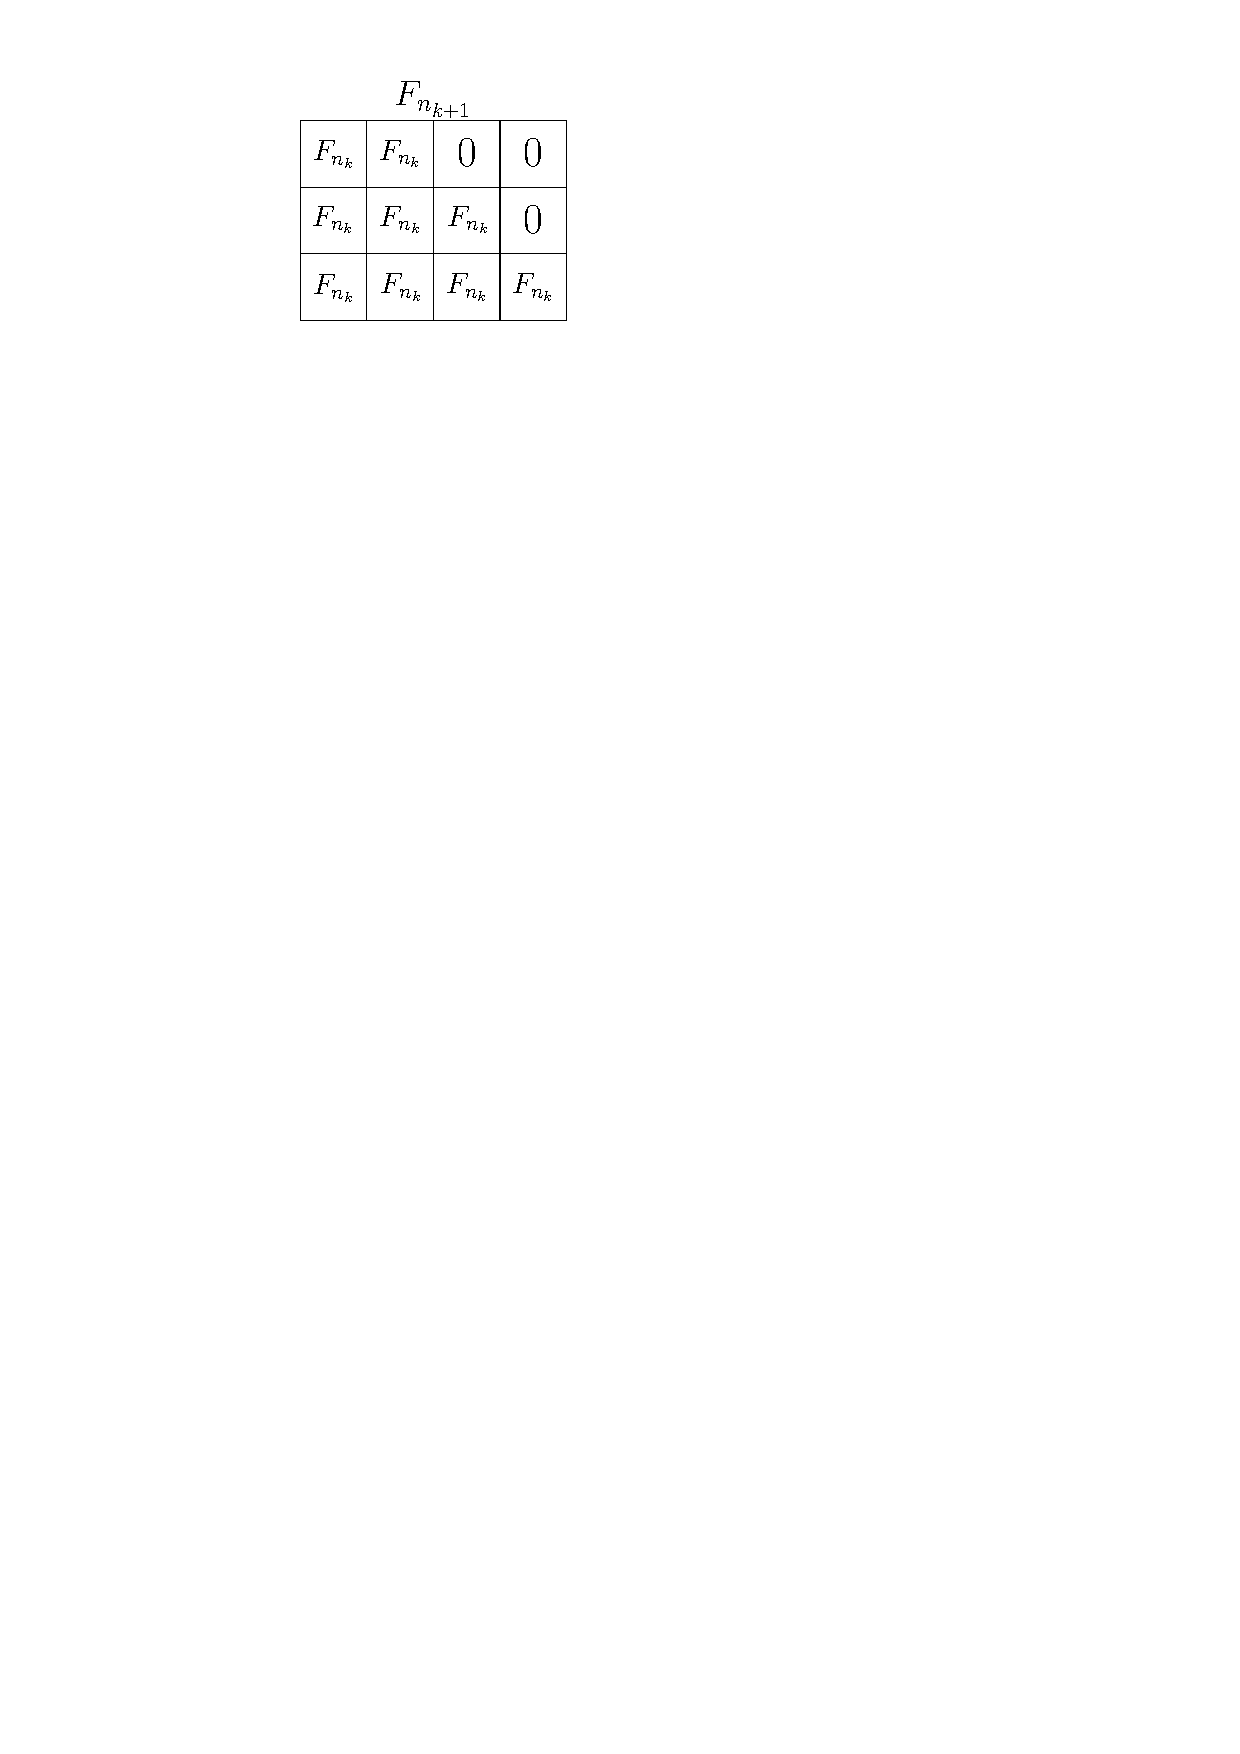
\includegraphics[scale=1.3]{../Graphics/obrazek_prox.pdf}
\caption{The $(k+1)$-th step of the construction of a pattern over $F_{n_{k+1}}$ in $x^{(k+1)}$ from the proof of Theorem \ref{thm:KriegerProximal}. We copy the pattern from $F_{n_k}$ to $m_k-r_k$ shifts of $F_{n_k}$ by some elements from $H_{n_k}$ and we fill the remaining places with zeros.}\label{fig:constr_prox}
\end{figure}


Let us now go back to the construction and justify that we can perform the step from $k$ to $(k+1)$.
%
Assuming that we have already constructed $x^{(k)}$ as a periodic configuration with period $H_{n_k}$, we construct $x^{(k+1)}$ as follows.
%
Intuitively: after choosing $n_{k+1}$, we copy the pattern from $F_{n_k}$ in $x^{(k)}$ over some (not all) shifts of $F_{n_k}$ contained in $F_{n_{k+1}}$ and then we fill with zeros the remaining places.
%
Finally, we copy the pattern from $F_{n_{k+1}}$ to the whole group $G$ using $H_{n_{k+1}}$.
%
When choosing  ${n_{k+1}}$ the goal is for the density of ones in $F_{n_{k+1}}$ to satisfy 
\[
\gamma<d_{k+1}\leq\frac{1}{2}(d_k+\gamma)<d_k .
\]
Hence two problems may appear, if we fill $F_{n_{k+1}}$ with too many zeros, then $d_{k+1}<\gamma$, and if we fill it with too little zeros, then $d_k$ might never converge to $\gamma$. Therefore we need to choose $n_{k+1}$ such that $F_{n_{k+1}}$ fits with a lot of copies of $F_{n_k}$ so that we can ``balance out'' the number of zeros just right.


Let us now write down the above idea formally.
%
By  Lemma~\ref{Cortez} we have that
\[
F_{n_{k+1}}=\bigsqcup\{F_{n_k}g:g\in F_{n_{k+1}}\cap H_{n_k}\}.
\]
We divide $F_{n_{k+1}}\cap H_{n_k}$ into two disjoint parts $S_k$ and $Z_k$ (to be specified later), and assign:
\[
x^{(k+1)}(gh) \defeq \begin{cases}
x(g) &\text{if } h\in S_k, \\
0 &\text{if } h\in Z_k, \end{cases} \quad \text{ for } g\in F_k.
\]
Having $x^{(k+1)}$ defined over $F_{n_{k+1}}$, we copy this pattern to $G$:
\[
x^{(k+1)}(gh) \defeq x^{(k+1)}(g) \quad \text{ for } g\in F_{n_{k+1}},\, h\in H_{n_{k+1}}.
\]
To finish the construction, it is enough to specify $S_k$ and $Z_k$. Denote
\[
m_k~\defeq~|F_{n_{k+1}}~\cap~ H_{n_k}|\quad\text{ and } \quad r_k\defeq|Z_k|.
\]
We will determine $r_k$.
Let $\eps_k := d_k-\gamma$ for every $k\in\N$. Notice that by conditions \eqref{d_k_decrease} and \eqref{dist_from_a} in the induction thesis we have $0<\eps_{k+1}<\frac{1}{2}\eps_k.$ Since
\[
d_{k+1} = \frac{m_k-r_k}{m_k}d_k,
\]
we obtain
\[
\eps_{k+1}=d_k-\gamma-\frac{r_k}{m_k}d_k = \eps_k - \frac{r_k}{m_k}d_k.
\]
Hence in conditions \eqref{d_k_decrease} and \eqref{dist_from_a} we require
\[
0< \eps_k - \frac{r_k}{m_k}d_k<\frac{1}{2}\eps_k,
\]
which is equivalent to 
\[
\frac{\eps_k}{2d_k}m_k<r_k<\frac{\eps_k}{d_k}m_k.
\]
%
Therefore it is enought to choose $n_{k+1}$ such that $F_{n_{k+1}}$ is so large that there exists an integer between $\frac{\eps_k}{2d_k}m_k$ and $\frac{\eps_k}{d_k}m_k$. This is possible, since $\eps_k$ and $d_k$ are fixed positive numbers and $m_k \to \infty$ as we go with $n_{k+1}$ to infinity. We take this integer to be $r_k$, i.e., the number of copies of $F_{n_k}$ in $F_{n_{k+1}}$ that we fill with zeros.
%
We refer to Figure~\ref{fig:constr_prox} for a graphical explanation of this construction.

From now on, for simplicity of notation we assume that $n_{k}=k$ for all $k \in \N$.
%
The next step is to prove that $\htop(\subord{Z)}=\gamma\log2$.
%
To this end, fix $n\in\N$ and denote
\[
\subord{Z}^{(n)} \defeq \{y\in\{0,1\}^G:\exists z\in \closure{Gx^{(n)}} \,\,\,\forall g\in G \,\,\,\, y(g)\leq z(g) \} .
\]
Notice that 
\begin{equation*}\label{eq:zawieranie_daszkow}
\subord{Z}\subseteq\subord{Z}^{(n)}.
\end{equation*}
Indeed,  $x(g)\leq x^{(n)}(g)$ for every $g\in G$. Thus $x\in \subord{Z}^{(n)}$. 
This and Lemma \ref{lem:subordinate_periodic_entropy} imply that
\begin{equation*}\label{eq:entropy_ineq}
\htop(\subord{Z})\leq\htop(\subord{Z}^{(n)})=d_n \log2.
\end{equation*}
Therefore, since $n$ was arbitrary, we have
\[
\htop(\subord{Z})\leq \gamma\log 2.
\]
On the other hand for every $n\in\N$ it holds
\[
\inmodul{\lang_{F_n}(\subord{Z})}\geq 2^{|F_n|d_n}.
\]
Hence 
\[
\frac{1}{|F_n|}\log\inparen{\inmodul{\lang_{F_n}(\subord{Z})}}\geq d_n\log 2\geq \gamma\log 2,
\]
and passing with $n$ to $\infty$ we consequently have $ \htop(\subord{Z})\geq \gamma\log 2$.
%



Finally we are left with the task of proving that $(\subord{Z},G)$ is proximal.
%
Before we proceed with the proof, recall that the metric $\rho$ on $\{0,1\}^G$ is defined as:
\[
\rho(z,y)=2^{-k}\quad\text{ with } \quad k= \min\inbrace{i\in\N: z(g_i)\neq y(g_i)},
\]
where $(g_1,g_2,\ldots)$ is any bijective enumeration of elements of $G$. It will be convenient for us to assume that this enumeration is consistent with the \Folner sequence in the following sense:
\[
 \exists n\in\N~~~~ g_l\in F_n~~ \mbox{ and }~~ g_k\notin F_n \quad \implies \quad l<k.
\]
In other words, elements in $F_0$ go first, next elements in $F_1\setminus F_0$, next in $F_2\setminus F_1$ and so on.

Now, observe that by the construction of $x$, it is clear that for every $n\in \N$ we have $x_{F_n}=x_{F_ng}$ for infinitely many $g\in G$. 
%
Hence, applying Lemma \ref{lem:subord-transit2} we obtain that $\subord{Z}$ is transitive.
%
Let $z\in\subord{Z}$ be such that $\closure{Gz}=\subord{Z}$.
%
We now apply Theorem \ref{thm:minimal-synd} to show that $\{0^G\}$ is the only minimal subsystem of $\subord{Z}=\closure{Gz}$, i.e., $m(z)=1$. 
%
For this, we need to show that for every $\eps>0$ the set 
\[
S\defeq\inbrace{g\in G: \rho(gz,0)< \eps}
\]
is syndetic. Fix $\eps>0$. Then there exists an $n\in\N$ such that $|F_n|>\frac{1}{\eps}$.
%
By the construction of $x$, there exists $h_0\in H_n$ such that 
\[
x_{F_nh_0}\equiv 0.
\]
Then for every $h\in H_{n+1}$ we have
\[
x_{F_nh_0h}\equiv 0.
\]
But $z\leq x$, hence for every $h\in H_{n+1}$ we also have
\[
z_{F_nh_0h}\equiv 0.
\]
Thus
\[
\rho(h_0hz,0)<\eps \quad \text{ for } h\in H_{n+1},
\]
which means that $h_0H_{n+1}\subseteq S$. Therefore taking $F=F_{n+1}h_0^{-1}$ we obtain
\[
FS\supseteq Fh_0H_{n+1}=F_{n+1}h_0^{-1}h_0H_{n+1}=F_{n+1}H_{n+1}=G. 
\]
\noindent Consequently, the claim holds and $\subord{Z}$ indeed is a proximal system with $0^G$ being its only fixed point. 
\end{proof}

\begin{rem}\label{rem:prox_realiz_general}
%
The general version of Theorem \ref{thm:KriegerProximal} (i.e., for arbitrary alphabet $\alf=\{0,1,\ldots, k-1\}$) can be obtained by repeating the proof of Theorem \ref{thm:KriegerProximal} with a small modification: in the construction of $x$ we replace $1$'s by $(k-1)$'s. 

For this proof to go through we need a new version of Theorem \ref{thm:entropy-density}, yet a complete generalization is not necessary. It is sufficient to prove that if a subshift $Z\subseteq\{0,k-1\}^G \subseteq \alf^G$ is such that $\htop(Z)=0$, then the entropy of the subordinate shift $\subord{Z}\subseteq\alf^G$ is given by
\[
\htop(\subord{Z})=\log (k)\lim_{n\to\infty}\frac{1}{|F_n|}\max\inbrace{\sum_{g\in F_n} \frac{w(g)}{k-1}: w\in \mathcal B_{F_n}(Z)}.
\]
This, however, can be argued in the same way as for the binary alphabet, since only two characters: $0$ and $k-1$ play a role.
\end{rem}


